%% LyX 2.0.8.1 created this file.  For more info, see http://www.lyx.org/.
%% Do not edit unless you really know what you are doing.
\documentclass[12pt,british]{article}
\usepackage{mathptmx}
\usepackage[T1]{fontenc}
\usepackage[latin9]{inputenc}
\usepackage[a4paper]{geometry}
\geometry{verbose,tmargin=2cm,bmargin=2cm,lmargin=2cm,rmargin=2cm}
\pagestyle{plain}
\setcounter{secnumdepth}{5}
\setcounter{tocdepth}{5}
\usepackage{bm}
\usepackage{graphicx}

\makeatletter

%%%%%%%%%%%%%%%%%%%%%%%%%%%%%% LyX specific LaTeX commands.
%% A simple dot to overcome graphicx limitations
\newcommand{\lyxdot}{.}


%%%%%%%%%%%%%%%%%%%%%%%%%%%%%% User specified LaTeX commands.
\usepackage{color}
\newcommand{\nicefrac}[2]{\ensuremath ^{#1}\!\!/\!_{#2}}
\usepackage { fancybox}

\renewcommand{\floatpagefraction}{0.95}
\renewcommand{\textfraction}{0}
\renewcommand{\topfraction}{1}
\renewcommand{\bottomfraction}{1}

\RequirePackage{tweaklist}
\renewcommand{\itemhook}
{
    \setlength{\topsep}{3pt}
    \setlength{\parskip}{0pt}
    \setlength{\parsep}{0pt}
    \setlength{\partopsep}{0pt}
    \setlength{\itemsep}{0pt}
    \setlength{\labelwidth}{10pt}
    \setlength{\leftmargin}{\labelwidth}
}

\renewcommand{\enumhook}
{
    \setlength{\topsep}{3pt}
    \setlength{\parskip}{0pt}
    \setlength{\parsep}{0pt}
    \setlength{\partopsep}{0pt}
    \setlength{\itemsep}{3pt}
    \setlength{\labelwidth}{10pt}
    \setlength{\leftmargin}{\labelwidth}
}

\renewcommand{\descriptionlabel}[1]{\parbox{\leftmargin}{\raggedleft #1.~}}

\makeatother

\usepackage{babel}
\begin{document}

\title{icoFoamH - incompressible solver on a C-grid with a Hodge operator}

\maketitle
The continuous equations solved are the incompressible Euler equations
\begin{equation}
\frac{\partial\mathbf{u}}{\partial t}+\nabla\cdot\left(\mathbf{u}\mathbf{u}\right)=-2\bm{\Omega}\times\mathbf{u}-\nabla p\label{eq:mom}
\end{equation}
subject to the constraint
\begin{equation}
\nabla\cdot\mathbf{u}=0\label{eq:divFree}
\end{equation}
where $\mathbf{u}$ is the velocity and $p$ is the pressure. The
numerical solution uses the prognostic variable
\begin{equation}
V_{f}=\mathbf{u}_{f}\cdot\mathbf{d}_{f}
\end{equation}
where $\mathbf{u}_{f}$ is the velocity on face $f$ and $\mathbf{d}_{f}$
is the vector between cell centres either side of face $f$.

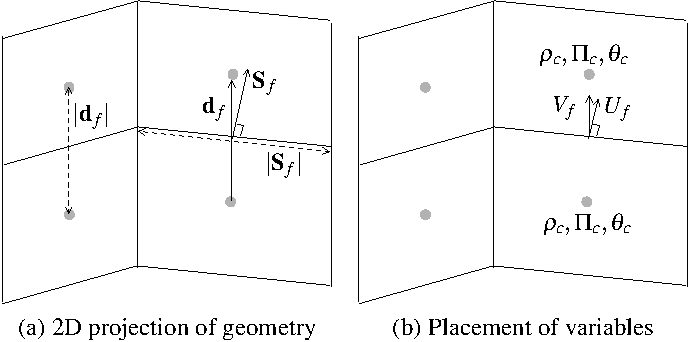
\includegraphics{/home/hilary/latex/myPapers/ExnerFoam/submit2/geometryVariables}

We also define a diagnostic variable for the volumetric flux across
face $f$: 
\begin{equation}
U_{f}=\mathbf{u}\cdot\mathbf{S}_{f}
\end{equation}
where $\mathbf{S}_{f}$ is the normal vector to face $f$ with magnitude
equal to the area of face $f$. The pressure, $p$, is an auxiliary
variable. 

We use the convection that $U$ is a vector of all values of $U_{f}$
on all faces and $V$ is a vector of all values of $V_{f}$.

The numerical solution uses projection method: the momentum equation
(\ref{eq:mom}) is solved without the pressure gradient term to find
an intermediate value of the velocity, then this velocity is projected
into divergence free space by solving a pressure equation and then
adding the pressure gradient term to the intermediate velocity. To
discretise the momentum equation (\ref{eq:mom}), we take the dot
product with $\mathbf{d}$:
\begin{equation}
\frac{\partial V}{\partial t}+\left(\nabla\cdot\left(\mathbf{u}\mathbf{u}\right)\right)\cdot\mathbf{d}=-\left(2\bm{\Omega}\times\mathbf{u}\right)\cdot\mathbf{d}-\nabla_{d}p\label{eq:momDotd}
\end{equation}
where $\nabla_{d}p=\mathbf{d}\cdot\nabla p$ so that the simplest
discretisation of $\nabla_{d}p$ is simply the difference between
the two values of the pressure, $p$, either side of the face. We
can now discretise in time using trapezoidal-implicit time-stepping
with deferred correction of explicit terms:
\begin{equation}
V^{n+1}=V^{n}+(1-\alpha)\Delta t\left(\frac{\partial V}{\partial t}\right)^{n}-\alpha\Delta t\left\{ \left(\nabla\cdot\left(\mathbf{u}\mathbf{u}\right)^{\ell}\right)\cdot\mathbf{d}+\left(2\bm{\Omega}\times\mathbf{u}^{\ell}\right)\cdot\mathbf{d}+\nabla_{d}p^{n+1}\right\} \label{eq:momD}
\end{equation}
where $\Delta t$ is the time-step, $\alpha$ is the off-centering
parameter and $\ell$ represents values of variables at the most recent
iteration within each time-step but not at the latest time since they
are not solved for implicitly. Next we define an intermediate value,
$V^{i}$, (which shares the same storage as $V$), using explicitly
defined values:
\begin{equation}
V^{i}=V^{n}+(1-\alpha)\Delta t\left(\frac{\partial V}{\partial t}\right)^{n}-\alpha\Delta t\left(\nabla\cdot\left(\mathbf{u}\mathbf{u}\right)^{\ell}\right)\cdot\mathbf{d}.\label{eq:Vi}
\end{equation}
Variables $V$, $V^{i}$ and $\partial V/\partial t$ share the same
boundary conditions at zero flux boundaries (ie they are all set to
zero at zero flux boundaries). Next we apply the Hodge operator, $H$,
to find the intermediate value of the flux, before pressure gradients
are applied:
\begin{eqnarray}
U^{i} & = & HV^{i}-\alpha\Delta t\ 2\left(\bm{\Omega}\times\mathbf{u}^{\ell}\right)\cdot\mathbf{S}.\\
 & = & HV^{i}-\alpha\Delta t\ 2\left(\mathbf{S}\times\bm{\Omega}\right)\cdot\mathbf{u}^{\ell}.
\end{eqnarray}
Alternatively, if we had applied the Hodge operator to $V^{n+1}$
from eqn (\ref{eq:momD}) we would get an equation for the flux:
\begin{equation}
U^{n+1}=U^{i}-\alpha\Delta t\ H\nabla_{d}p^{n+1}.\label{eq:flux}
\end{equation}
We require the velocity field to be divergence free at every time-step,
ie $\nabla\cdot U^{n+1}=0$ where $\nabla\cdot U^{n+1}$ represents
the discrete calculation of $\nabla\cdot\mathbf{u}$ and is calculated
as:
\begin{equation}
\nabla\cdot U=\frac{1}{v_{c}}\sum_{f\in c}U_{f}\label{eq:divU}
\end{equation}
where $v_{c}$ is the volume of cell $c$ and $f\in c$ means all
the faces, $f$, of cell $c$. Therefore, substituting eqn (\ref{eq:flux})
into $\nabla\cdot U=0$ gives:
\begin{equation}
\nabla\cdot U^{i}-\alpha\Delta t\nabla\cdot H\nabla_{d}p^{n+1}=0.\label{eq:p}
\end{equation}
This is the pressure equation, a Helmholtz equation that can be solved
implicitly for $p$. In order to simplify the construction of the
matrix for the implicit solution of (\ref{eq:p}), we can separate
$H\nabla_{d}p$ into diagonal and off-diagonal parts:
\begin{eqnarray}
H\nabla_{d}p & = & H_{d}\nabla_{d}p+H_{off}\nabla_{d}p\\
 & = & \frac{|\mathbf{S}|}{|\mathbf{d}|}\nabla_{d}p+H_{off}\nabla_{d}p
\end{eqnarray}
and only solve the diagonal part implicitly. Then $U^{i}$ can be
re-defined to include the off diagonal part of the Hodge operator:
\begin{equation}
U^{i}=HV^{i}-\alpha\Delta t\ 2\left(\mathbf{S}\times\bm{\Omega}\right)\cdot\mathbf{u}^{\ell}-\alpha\Delta t\ H_{off}\nabla_{d}p^{\ell}
\end{equation}
leaving the pressure equation simpler:
\begin{equation}
\nabla\cdot U^{i}-\alpha\Delta t\nabla\cdot\frac{|\mathbf{S}|}{|\mathbf{d}|}\nabla_{d}p^{n+1}=0.\label{eq:pDiag}
\end{equation}
Equation (\ref{eq:pDiag}) is solved implicitly for $p$ and then
we can calculate divergence free velocity components, $U$ and $V$
(the back-substitution step):
\begin{eqnarray}
V^{n+1} & = & V^{i}-\alpha\Delta t\left\{ \left(2\bm{\Omega}\times\mathbf{u}^{\ell}\right)\cdot\mathbf{d}+\nabla_{d}p^{n+1}\right\} \\
U^{n+1} & = & U^{i}-\alpha\Delta t\ H\nabla_{d}p^{n+1}.
\end{eqnarray}
In order to ensure no flow at boundaries, geostrophic balance can
be imposed, ie:
\begin{equation}
\nabla_{d}p=\left(2\bm{\Omega}\times\mathbf{u}^{\ell}\right)\cdot\mathbf{d}
\end{equation}
at boundaries. 

\bibliographystyle{abbrvnat}
\bibliography{numerics}

\end{document}
